\documentclass{article}
\usepackage{amsmath}
\usepackage{ctex}
\usepackage{graphicx}
\usepackage{tikz}

\usepackage{algorithm}
\usepackage{algorithmicx}
\usepackage{algpseudocode}

\usepackage{geometry}
\geometry{left=2cm, right=2cm, top=1.5cm,bottom=1.5cm}

\title{数据结构第三次项目\\路由问题}
\author{陈小羽\ 2016060106020\ (单刷)}
\date{}

\begin{document}
\maketitle
\clearpage
\tableofcontents
\clearpage


\section{题目要求}
	\paragraph{}
		一般的网络都有一个网关(外接路由器)与Iternel网相连,负责获得外网
		发送至内部单位的信息,并转发至内网。现在假设内网有一些机器,每次
		能告诉网关自己和周围机器的连接情况,现在需要给网关设计一个算法,
		使得网关在收到连接信息之后,可以找到到达每个设备的最优的路径
		(路由表)
\section{选择算法和实现}
	\subsection{最短路径算法}
		\paragraph{}
			首先我们把这个问题转化为图论中的问题。为了达到这个目的,
			我们可以令原来连接设备的网线作为图中的边,令原来两个设
			备之间连接的优劣程度作为边的边权,令设备作为图中的点,
			并设网关为点1。我们把这个图记做$G = (V, E)$,其中,
			$V$表示点集, $E$表示边集。
		\paragraph{}
			然后,原来的问题就转化为了求图中1点到其他的点的最短路的
			问题。因为题目中出现的这种场景导致边权不可能出现复数,
			所以,我们可以使用Dijkstra算法来解决这个问题。
		\paragraph{}
			因为Dijkstra算法的过程比较复杂,不太好用语言描述清楚,
			所以在这篇文章中,我们选择直接给出伪代码。具体参见
			\textbf{算法\ref{algo1}}(在这个算法实现中,我使用了优先队列来优,
			化算法在渐近意义下的复杂度,但是并没有给出优先队列算法
			的细节,具体算法,我会在后面的章节中给出)。
			\begin{algorithm}[!h]
				\caption{Dijkstra算法(\ref{algo1})}
				\begin{algorithmic}[1]
					\State{int dis[maxn]}
					\Comment{用于储存起点到这个点的距离}
					\State{int pre[maxn]}
					\Comment{用于储存这个结点在最短路中的前驱结点}
					\State{PriorityQueue q}
					\Comment{优先队列(用于优化Dijkstra算法), 优先弹出距离小的元素}
					\Function {Dijkstra} {起点$s$, 点的个数$n$}
						\Comment{这个函数会求出dis和pre两个数组}
						\For{ i $\gets$ 1 : n }
						\Comment{初始化数组}
							\State{pre[i] = -1}
							\State{dis[i] = $\infty$}
						\EndFor
						\State{dis[1] = 0}
						\State{q $\gets \emptyset$}
						\State{q.push(s, 0)}
						\Comment{起点入队, 距离为0}
						\While{q非空}
							\State{ Front $\gets$ q.pop() }
							\Comment{这里的Front是一个包含id和dis两个变量的结构}
							\If{Front.dis < dis[Front.id]}
							\Comment{一个结点有可能重复入队,我们取距离最小的一个}
								\State{continue}
							\EndIf
							\For{每一个和Front.id相连的结点to}
								\If{dis[to] > Front.dis + $edge(Front.id, to).length$}
								\Comment{$edge(i,j)$表示的是一个边}
									\State{dis[to] $\gets$ Front.dis + $edge(Front.id, to).length$}
									\State{q.push(to, dis[to])}
								\EndIf
							\EndFor
						\EndWhile
					\EndFunction
				\end{algorithmic}
				\label{algo1}
			\end{algorithm}
		\paragraph{}
			下面让我们来分析一下这个算法的复杂度。首先,算法会把图中的所有的边都给遍历
			一遍。并且,Dijkstra算法严格保证了每一个点出队之后就再也不会再次入队了。
			所以总的时间复杂度为$\mathcal{O}\left((|V|+|E|)\times T(operation)\right)$
			这个$T(operation)$表示的是优先队列单次操作的复杂度。
			所以又有$T(operation) = \log (N)$。最后因为每一条边都可能会导致一个点入队,
			所以队列中的总的结点数最多为$|V| + |E|$个。所以,综合所有以上这些信息的话,
			我们可以得出结论:总的时间复杂度为$\mathcal{O}\left((|V|+|E|)\log (|V|+|E|)\right)$。
			这个结果相当于最原始的$\mathcal{O}(|V||E|)$已经相当不错了。
	\subsection{优先队列(小根堆)}
		\paragraph{}
			为了对原始版本的Dijkstra算法进行优化,我们在之前使用到了小根堆。在这里,
			我们来讨论一下小根堆具体的一些细节。
		\paragraph{}
			小根堆内部维护了一颗完全二叉树。这个完全二叉树上的元素要保证父亲结点储存的值要
			小于儿子结点储存的值。然后,这个小根堆要支持插入一个元素的操作和删除/查询最小
			元素的操作。因为它支持的操作的特殊性,小根堆有时又被称为优先队列, 即队首元素
			是整个队列中的最小的元素。下面我们来看一下具体的操作要怎么实现,以及他们需要
			花费的代价。因为堆的操作相对简单,所以我们直接采用文字叙述。
		\paragraph{插入q.push()}
			将要加入的元素放到完全二叉树的最后一个位置,然后不断的把这个元素和它的父亲
			结点比较,如果这个元素小于父亲结点的话,就将这个元素和父亲结点交换,否则,
			插入,结束。因为堆是完全二叉树,深度为$\log N$。所以插入操作最多进行$\log N$
			次比较和交换。所以,插入操作的复杂度为$\mathcal{O}(\log N)$, 其中$N$为堆中
			元素的个数。
		\paragraph{弹出最小元素q.pop()}
			显然,完全二叉树的根就是最小的元素。然后,我们只需要考虑如何删除这个元素就可以了。
			我们可以将完全二叉树的最后一个元素拿到根结点覆盖原来的根节点。然后将这个结点
			往下放,把这个结点儿子中最小的,比这个结点小的结点和这个结点换,然后不停的
			迭代,直到这个结点没有满足要求的儿子结点。因为树的深度的关系,这个操作的
			复杂度,显然也是$\mathcal{O}(\log N)$的。
		\paragraph{}
			下面给出具体的程序:
			\begin{center}
			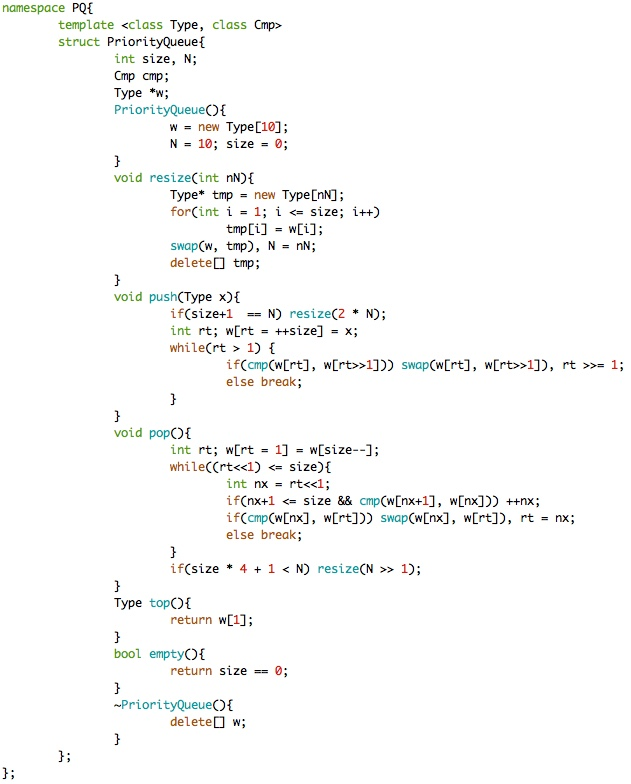
\includegraphics[width = 15cm]{pq.jpeg}\\
			\end{center}
			我实现了动态的堆。方法是:当堆满时,将这个堆重建,重新申请大小为$2N$的内存空间。
			当堆中元素个数小于$\frac{N}{4}$时,将堆重建,重新申请大小为$\frac{N}{2}$的内存
			空间。这种操作可以保证堆在内存中是连续的。而且这种看似暴力的操作,在均摊意义下,
			并不会对堆的渐近复杂度又任何影响。
	\subsection{生成路由表}
		\paragraph{}
			值得注意的是,上面的Dijkstra算法只能计算出dis和pre连个数组的值,但是这两个数组里面
			的值还算不上是真正的路由表。所以,我们还需要设计一个可以打印出路由表的算法。
			为了代码实现的简洁性,我选择了一个递归的算法来实现这个功能,具体可以看下面给出
			的\textbf{伪代码\ref{algo2}}。
			\begin{algorithm}[!h]
				\caption{打印路由表(伪代码\ref{algo2})}
				\begin{algorithmic}[1]
					\Function{printRoad}{结点x}
					\Comment{打印出以x结尾的路径}
						\If{$x \not= 1$}
						\Comment{到达了1点,递归结束}
							\State{printRoad(pre[x])}
						\EndIf
						\State{输出 x}
					\EndFunction
					\Function{printTable}{}
					\Comment{printRoad的具体使用方法的示例}
						\For{$i \gets 2:n$}
							\State{printRoad(i), 换行}
						\EndFor
					\EndFunction
				\end{algorithmic}
				\label{algo2}
			\end{algorithm}
	\subsection{小结}
		\paragraph{}
			有了前面说的算法,就可以上机实现程序了。
			具体程序运行的效果如下图。
			\begin{center}
			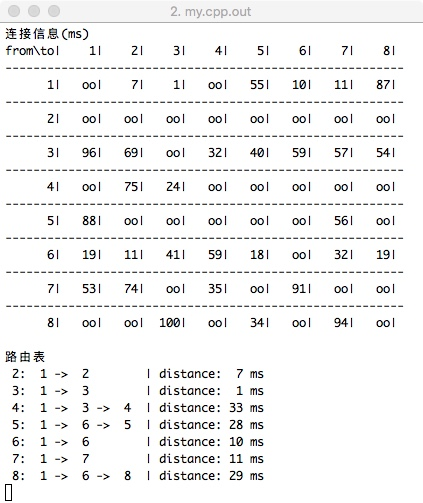
\includegraphics[width = 8cm]{runtime.jpeg}\\
			\end{center}
			其中,连接信息是随机生成的,其原理显然不是这篇文章乃至这次实验的重点。
			每次敲击一下键盘,程序就会更新连接信息并且计算出相应的路由表。
		\paragraph{}
			下面,实现程序之后,就到了测试的环节。
\section{测试}
	\subsection{测试小根堆}
		\paragraph{}
			因为这个程序中,小根堆是我自己手动实现的。所以在测试其他位置的问题之前,首先要
			测试小根堆写对没有。这种东西最好的测试方法就是将待测的代码和保证正确的代码
			运行在同一组输入上,然后比较输出即可。
		\paragraph{}
			好在STL中原生支持一个优先队列,这个模板类被包含在<queue>这个头文件中。
			所以,我们将原来的优先队列换成STL实现的优先队列就可以了(其他一些地方也需要改,
			这里就不一一说明了)。
			\begin{center}
			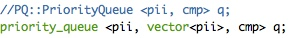
\includegraphics[width = 8cm]{change.jpeg}\\
			\end{center}
		\paragraph{}
			因为我的计算机是Unix环境,所以我使用bash和python实现了一个简单的脚本,可以
			用来测试程序的正确性。
			\begin{center}
			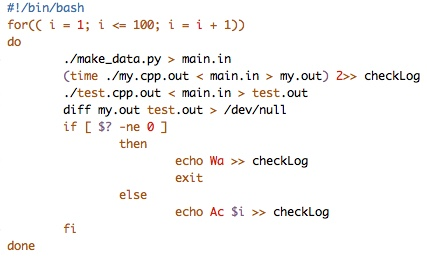
\includegraphics[width = 10cm]{check.jpeg}\\
			\end{center}
			他的作用就是生成随机的数据喂给两个程序,然后检测这两个程序的输出是否相同。
			经过测试可以发现,对于这随机的100组数据,两个程序得到了完全相同的输出。
			所以,我们有理由相信,小根堆的算法和实现是正确的。
			\begin{center}
			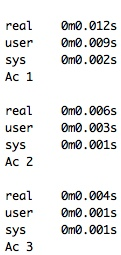
\includegraphics[width = 3cm]{log.jpeg}\\
			\end{center}
			另外还可以说明,这个算法运行起来是十分迅速的。
	\subsection{测试Dijkstra算法}
		\paragraph{}
			对于Dijkstra算法,我们就没有这么好的方式了。所以我们只有使用程序生成一些样例
			然后比较手动计算出的结果和程序是否是相同的。为了方便手动计算最短路,我使用了
			贝尔实验室开发的一个图形化软件,名字叫做:graphviz。这个软件有一个网页版的,
			网址是:http://www.webgraphviz.com 。我可以使用这个程序生成人类友好的图,
			以此来方便我进行手动计算。下面给出了一些测试用例。
		\paragraph{test1, n = 3}
			\begin{center}
			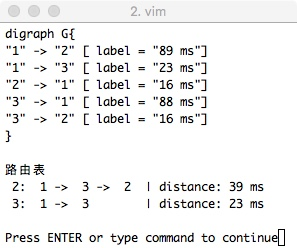
\includegraphics[width = 8cm]{data3.jpeg}
			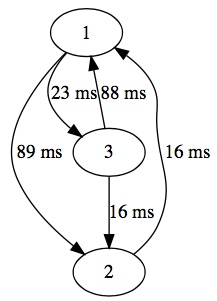
\includegraphics[width = 5cm]{data3viz.jpeg}
			\end{center}
		\paragraph{test2, n = 5}
			\begin{center}
			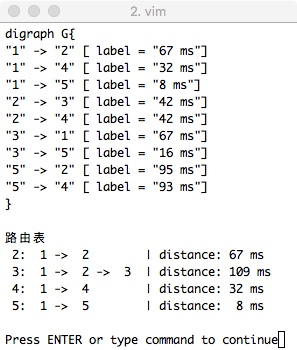
\includegraphics[width = 8cm]{data5.jpeg}
			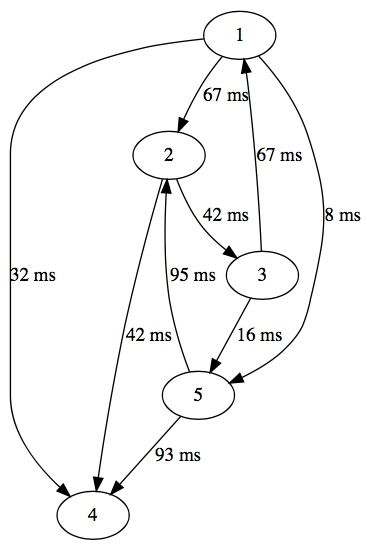
\includegraphics[width = 5cm]{data5viz.jpeg}
			\end{center}
			\clearpage
		\paragraph{test3, n = 5}
			\begin{center}
			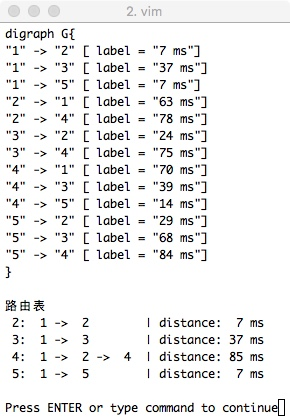
\includegraphics[width = 8cm]{data51.jpeg}
			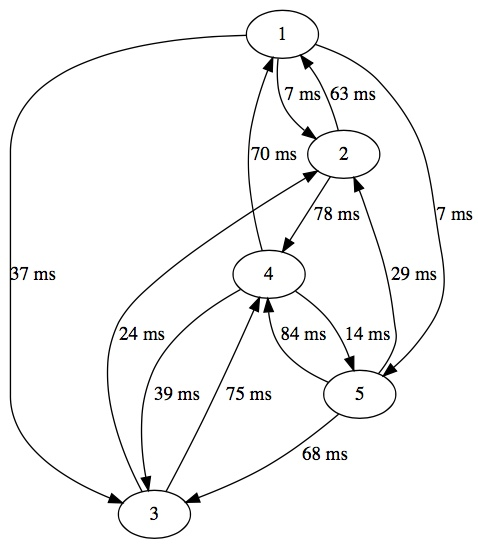
\includegraphics[width = 8cm]{data51viz.jpeg}
			\end{center}
		\paragraph{test4, n = 5}
			\begin{center}
			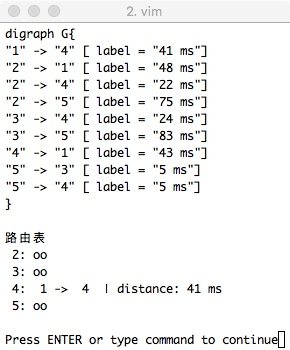
\includegraphics[width = 8cm]{data52.jpeg}
			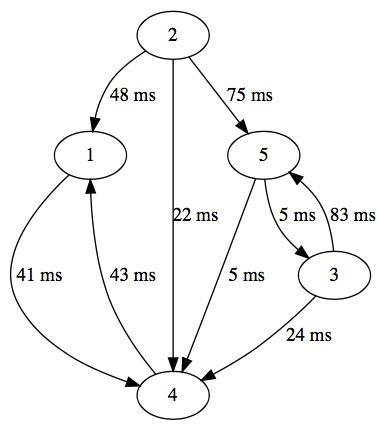
\includegraphics[width = 8cm]{data52viz.jpeg}
			\end{center}
			\clearpage
		\paragraph{test5, n = 8}
			\begin{center}
			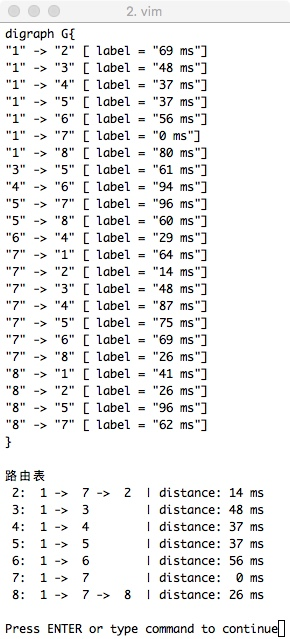
\includegraphics[width = 5cm]{data8.jpeg}
			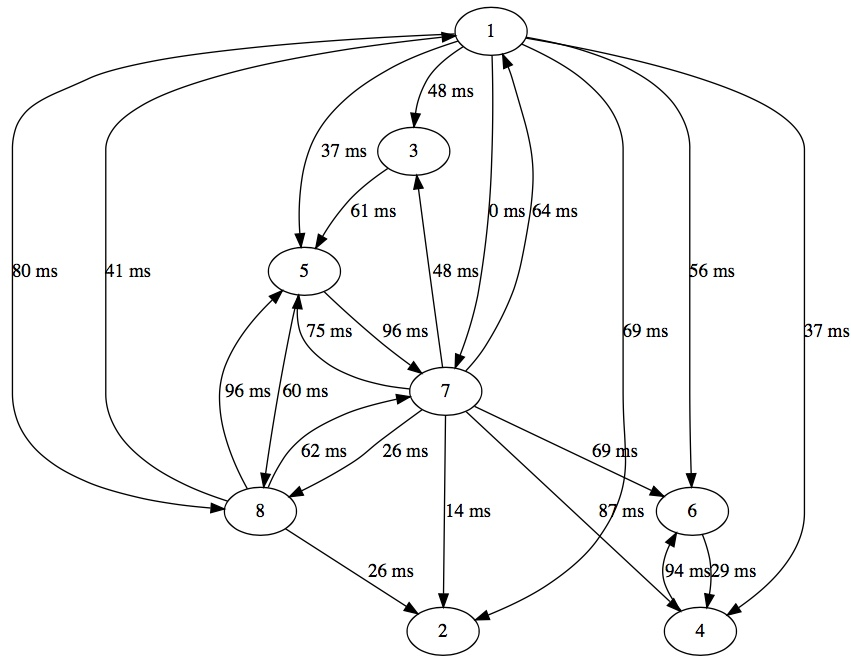
\includegraphics[width = 11cm]{data8viz.jpeg}
			\end{center}
			\clearpage
	\subsection{小结}
		\paragraph{}
			综合上面的各项测试数据,我们不难断定,这个程序已经不再怎么可能有什么大问题了。
			因为这个程序其他的位置,为了模拟网络环境的随机性,本来就是用了一些随机的算法,
			用于生成连接信息,所以,就算有一些小问题,也不会对最终的结果产生致命的影响。 \\
			至此,测试工作圆满结束:-)
\section{感想与收获}
	\paragraph{}
		通过这一次的数据结构作业,我又更加熟悉了小根堆的写法,还有Dijkstra算法的写法。
		通过测试,我尝试使用了graphviz来测试程序。通过写作文档练习了\LaTeX{}的使用方法。
		感觉这一次的作业从多个方面训练了我自己。虽然涉及到的算法略显简单,但是我借此机会
		磨练了其他方面的技巧。感觉收获很多。
\end{document}
